\documentclass[smallextended]{svjour3}       % onecolumn (second format)
%\documentclass[twocolumn]{svjour3}          % twocolumn

\smartqed  % flush right qed marks, e.g. at end of proof

\usepackage{graphicx}

\begin{document}

\title{Exploring and optimising infectious disease policies with a stylised agent-based model}
%\subtitle{Do you have a subtitle?\\ If so, write it here}

\titlerunning{Exploring and optimising infectious disease policies}        % if too long for running head

\author{Jeonghwa Kang          \and
        Juste Raimbault
}


\institute{J. Kang \at
              CASA, UCL \\
           \and
           J. Raimbault \at
              LASTIG, IGN-ENSG\\
              \email{juste.raimbault@ign.fr}
}

%\date{Received: date / Accepted: date}
% The correct dates will be entered by the editor


\maketitle

\begin{abstract}
The quantitative study of the spread of infectious diseases is a crucial aspect to design health policies and foster responsiveness, as the recent COVID-19 pandemic showed at an unprecedented scale. In-between abstract theoretical models and large-scale data driven microsimulation models lie a broad set of modelling tools, which may suffer from various issues such as parameter uncertainties or the lack of data. We introduce in this paper a stylised ABM for infectious disease spreading, based on the SIRV compartmental model. We account for a certain level of geographical detail, including commuting modes and workplaces. We apply to it a set of model validation methods, including global sensitivity analysis, surrogates, and multi-objective optimisation. This shows how such methods could be a new tool for more robust design and optimisation of infectious disease policies.
\keywords{Infectious disease \and Agent-based modelling \and Model exploration and validation \and Multi-objective optimisation}
\end{abstract}

% medicine and physiology ; computational social sciences
% Full paper (up to 12 pages): !!! - shorten

% Review 1
%  X. The paper presents an agent-based model of covid-19 diffusion and its analysis by a set of parameter space exploration methods. The main contribution of the article is the application of a classical set of exploration methods for a model dedicated to covid-19. Indeed, in itself the proposed model does not bring much compared to existing models: compared to many more descriptive agent-based models, it relies on many simplifying assumptions limiting the realism of the model and compared to mathematical models (compartment model), it does not allow to scale up. In addition, there is no validation of the model using real data, which limits its interest for decision support. The model parameter space exploration is interesting as an exercise, but given the limitations of the model, it does not provide essential information about covid-19 or covid-19 interventions.
%Some remarks:
%   X  Page 3: "which this researchs ABM is based upon" -> Not sure to understand what it means
%   X  Page 4: "Hence, the agents working in a big-sized companies are more likely to get infected than the agents working in mid and small-sized companies." -> Not sure about this hypothesis: if a large company has premises with a low density of people and well ventilated, the risk of contamination will be lower than in a small company but with cramped and poorly ventilated premises.
%   X Page 5: “An infected agent is then constantly introduced at a random location for the simulation's first month (30 days).” -> why integrating this dynamic?
%   X Page 5: “A certain number of people leave the area, and others come to stay in the area.” -> As the stylized model is already oversimplified, I am not sure to understand the interest of this dynamic.
%   X Page 5: “Infection rates are calculated based on the values of the global, patch and turtle variables.” -> It is better to avoid concepts coming from Netlogo that cannot be understood by people who are not familiar with this platform.
%   X Page 5: “ccar = 10%" -> there is an error here
%   X Page 6: “cBig = 40%, cMedium = 35%, cSmall = 30%"  -> explanation of values not very convincing.
%   X  Page 6: “Furthermore, patients with cardiovascular diseases are known to be at high risk of getting an infection.” -> Is there a source for this? That having these diseases can increase the probability of severe symptoms, yes, that it influences the probability of infection, it is not sure.
%   X Page 6: “Mask & Cardio = 45%; No mask & Cardio = 15%;” -> there is an error here
%   X Page 6: “vaccines are the most effective preventive measure which can trigger a biological immune response to fight disease-causing organisms” -> The vaccine reduces the likelihood of severe symptoms. On the other hand, its effect on the number of contaminations is more debatable.
%   X Page 6: “The level of social distancing ranges from 1 to 3. Each level refers to a percentage value that reduces the contact rate by 5. Hence, the actual percentage value of the social distancing ranges from 5 to 15 percent.” -> This way of considering social distancing seems very abstract and provides little information about this type of intervention.
%   X Page 7: “The model is set to run over 125 times for every combination of the input parameter values, and the output parameters average values are obtained at the end." -> Why 125 replications?
%   X Page 10: Why using Random Forest algorithm?
%   X Most of Figures are too small and difficult to read.


% Review 2
%   X This paper presents an ABM for the spread of COVID-19 and shows how model parameters can be explored an optimized. Overall, I think this type of approach makes a lot of sense, and the sentivity analyses and multi-objective optimization are good additions to the commonly used approach for such models. The model is well explained. This being said, a number of problems remains:
%.  X In the current model, the operationalization of transportation does not seem appropriate. It mimicks the fact that a group of agents (e.g., bus users) all gather in the same place for a few hours every day, which is really not how people use transportation. The modeling of car transportation is really the same as saying that people stay home. In reality, the transportation network is very structured (for example, someone might take the same bus line to go to work, and this bus might be very central or not in the network, etc.). It would be interesting to consider the influence of transportation if spatial structure was explicitely modeled, but this is not the case now.
%.  X Another problem of the model is that it neglects household infections, although many studies have shown that they were very frequent.
%.  X In general, there are two approches when using such ABMs. Either one wants to show that, in theory, a particular mechanism might exist (say, the structure of public transports might impact the spread of covid-19). In such case, one can use a very stylized model, focusing on this particular mechanism, without having to calibrate to real data. Another approach is to design a very realistic model, if possible calibrated with real data, in order to make predictions and carefully optimize interventions. The model presented here is very stylized, however it is not used to draw theoretical expectations but to train a model for prediction and find optimal parameter values. I don't think it is reasonable to expect such a model to produce anything more than some qualitative insights. For the analyses presented here, realistic and calibrated models should proabably be used.
%.  X There are quite a few typos and grammar mistakes.


% Review 3
%.  X Even if the paper could be considered as yet another model on Covid, it is very interesting from a methodological point of view concerning on one hand the articulation in between different types of models and on the other hand concerning the global research process that is clear and very well described. The comparison in between different tools and approaches available nowadays to study models more deeply (surrogate, sensitivity analysis, multi-objective model optimisation) are very interesting and will provide fruitful discussions at the conference.



\section{Introduction}

The impact of one of the fatal epidemics in history, the Black Death, has led to the death of almost one-third of the population of Europe, and the most recent epidemic in the world today, COVID-19, is currently costing millions of valuable human lives \cite{glatter2021history}. Before the introduction of mathematical and computational modelling, humans had little knowledge on how to effectively control and minimise the spread of infectious diseases. Furthermore, the importance of forecasting the spread of diseases in recent years has become even more crucial as the world is rapidly globalising with increasing travel rates and distances \cite{saker2004globalization}. Beyond the health burden of epidemics, many dimensions of social systems are affected, with for example broad economic impacts \cite{boucekkine2021economics}. The current world is a highly complex system in which numerous dimensions play a role in decision-making \cite{bickley2021does}. Designing disease control strategies imply accounting for various interacting factors and finding a compromise between multiple objectives \cite{kaszowska2022immunity}.

The first modelling approach to disease spreading goes back to the 17th century as John Graunt conducted an empirical study on infections affecting individuals in various regions in Britain \cite{morabia2013epidemiology}. Bernouilli introduced in the 18th century an equation-based approach to studying the outbreak of the smallpox epidemic in Europe \cite{dietz2002daniel}. Most recent modelling approaches range from elaborated mathematical models to data-driven microsimulation models. The recent pandemic has shown the usefulness of quantitative modelling to evaluate policies, such as how to vaccinate the population \cite{bosetti2022epidemiology} or to evaluate which degree of lockdown is necessary.

Agent-based modelling are proposed by some researchers as a powerful tool to explore practical scenarios for decision-making when managing the spread of infectious diseases \cite{miksch2019should}. The classical epidemiological modelling relies on compartmental models, such as the SIR model (Susceptible, Infected, Recovered), with differential equations governing the evolution of the different compartments, or in some cases discrete-time equations \cite{ramani2004oscillating}. Recent extensions, such as the SEIRD model \cite{chowell2008seasonal}, include a more detailed description of disease stages. \cite{chumachenko2018agent} describe an agent-based model based on similar states for agents. The advantage of the ABM approach is that one can define for each agent characteristics such as location, age, and many other factors believed necessary in the model. Once the agents are defined with their own set of characteristics, they proceed through a set of rules which enable them to interact with other groups of agents within the simulation. Age groups have contact probabilities to simulate the interactions and infections. More details can be included in an ABM, such as wearing face masks or respecting social distancing \cite{minoza2021covid}. Furthermore, the infectious disease may interact with other chronic conditions, what can be accounted for in an ABM \cite{fekadu2021impact}.


We propose in this paper to explore the potential of model validation methods to design and optimise epidemiological policies. We introduce a stylised model for the spread of infectious diseases, which is hybrid in the sense that it lies halfway large data-driven models and abstract theoretical models. We account for geographical factors, in particular commuting and workplaces. We focus, as an illustration, for two policy factors, which are social distancing and face masks \cite{kwon2021association}, and vaccination \cite{bicher2022model}. Our main contribution is the application of state-of-the-art model sensitivity analysis and validation techniques \cite{raimbault2019methods} to such a stylised model, opening research perspectives to cases where data is lacking, model parametrisation is uncertain, or actors have not the ressources to implement a large scale model, but where accounting for spatial and social structure remains crucial. We do not provide directly actionable policy insights, but rather provide a proof-of-concept of the use of such techniques to extend model capabilities: since our model lies between simple but scalable compartment models and very complicated data-driven microsimulation models, it could in principle not be used to investigate scenarios and decision-making. Our approach allows reducing uncertainty on parameters and providing multi-objective optima for example, improving thus the applicability of the model.

A few examples of the application of such techniques to epidemiological models can be found in the literature. \cite{baquela2022optimising} utilise a multi-objective optimisation algorithm for the distribution of limited vaccines resources. \cite{wu2013sensitivity} review sensitivity analysis of infectious disease models. No systematic application of an umbrella of model validation methods can however be found.


The rest of this paper is organised as follows: we first describe the stylised agent-based model, we then apply model exploration and validation methods to it, and finally discuss the implications of our results.




\section{Model description}


\subsection{Rationale}

Our simulation model projects a real-life situation where agents commute from home to their designated workplaces via different modes of transportation on a fixed daily schedule. At the beginning of the simulation, the entire population is set to susceptible. Then, an infected agent is introduced daily for the first 30 days because if none of the infected agents gets introduced into the environment, the infection process does not happen. The infection then spreads through localised interactions between agents.


\subsection{Model setup and dynamics}

One main assumption of the model is that most human interactions occur while people travel and work (while home infections play a role in disease transmission, our model is built to focus on parameters linked to social distancing in transport and at work). Hence, the scenario is primarily about people commuting from home to their designated workplaces via different modes of transportation, closely depicting ordinary people's daily routine. The simulation of this model considers several essential assumptions. The entire duration of the simulation is set to 365 days. Each day is equivalent to 24 ticks. Hence, each tick is equivalent to an hour. A single day comprises three pre-defined phases: the 'Home-hour', 'Commute-hour and 'Work-hour' phases, as show in Fig.~\ref{fig:modeltrans}.

\begin{figure}
	\centering
	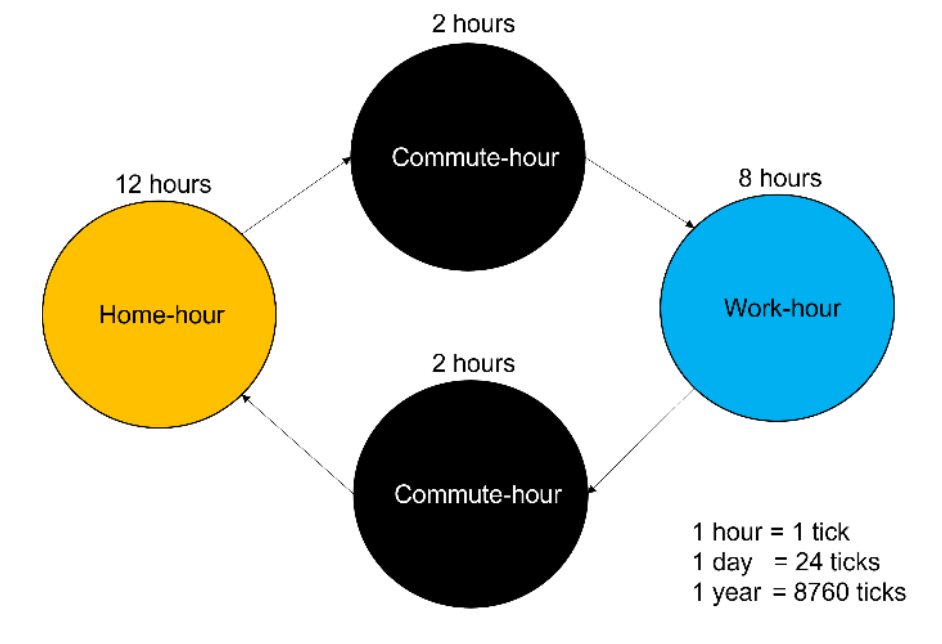
\includegraphics[width=\linewidth]{figures/ModelTransitions.png}
	\caption{Transitions between phases in the model.\label{fig:modeltrans}}
\end{figure}

During these phases, the movement of agents is completely randomised. No learning behaviour alternates the agents' movement in the simulation since it would be difficult for an individual to be fully aware of another agent's infection status. During the interaction, agents fall into one of the four states defined by the SIRV compartmental model. The SIRV model is an extended SIR model that accounts for the vaccination of the susceptible population \cite{poonia2022enhanced}. The agent states are shown in Fig.~\ref{fig:agentstates}.

\begin{figure}
	\centering
	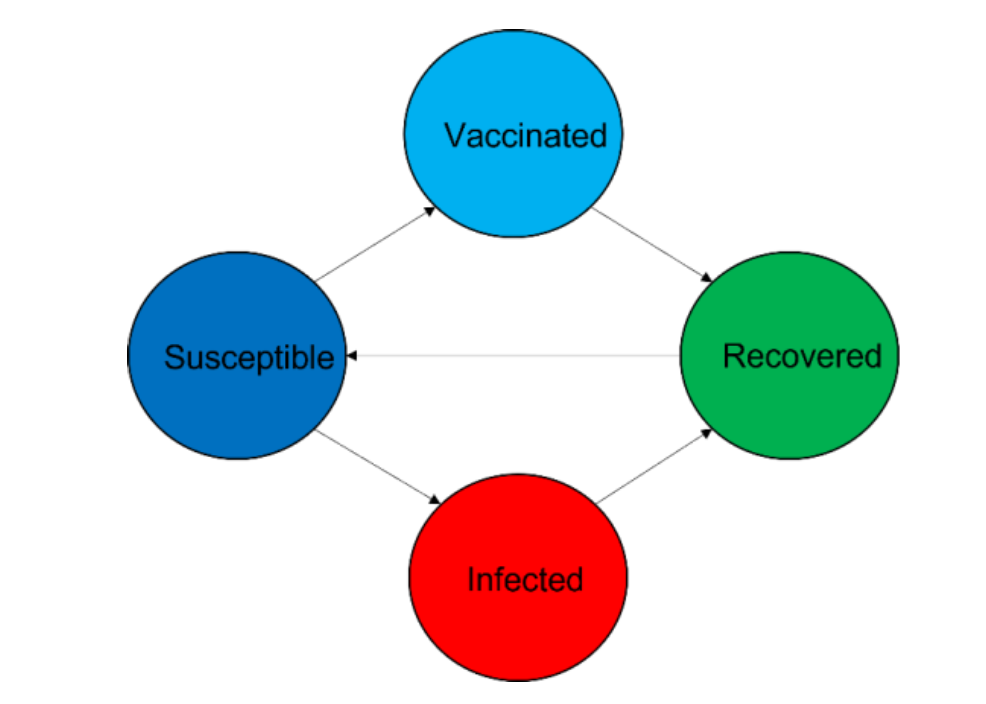
\includegraphics[width=\linewidth]{figures/AgentStates.png}	
	\caption{Agent states in the model\label{fig:agentstates}}
\end{figure}

Agents can interact with each other based on the state in which they fall. However, the interaction and infection processes are set to occur between the agents within the same patch only. The infection does not happen during the 'Home-hour' phase as this model does not consider social activities or household infections. During the 'Commute-hour' phase, an infected agent can only infect the susceptible agents that use the same mode of transportation as itself. It would be logically sensible that an infected agent commuting via train can only interact with and infect other susceptible agents commuting via the same mode of transportation. This same logic applies during the 'Work-hour' phase, where an infected agent can only interact with and infect other susceptible agents working in the same company. We include four modes of transportation in the model (metro, train, walking, car). The stylised way transportation is described allows avoiding the complexity of transport microsimulation (see e.g. \cite{axhausen2021modelling} for an adaptation of the MATSim framework to epidemiological modeling) while still accounting for transport processes. We furthermore consider stylised company size distributions (7 large companies, 4 medium sized, 4 small). There are total of fifteen companies which are randomly categorised into small, mid, and big-sized companies. The central assumption is that the bigger the company size, the more the human interactions involved. Hence, the agents working in a big-sized companies are more likely to get infected than the agents working in mid and small-sized companies (in practice, this assumption could be refined, as infections also depends on the size of the premises and on ventilation; simulating density and real-time interaction remains however out of the scope of our stylised approach).


At the beginning of the simulation, $N = 1500$ susceptible agents are randomly distributed in the simulation environment. The variable values for the agents, such as the transportation and company, are randomly assigned during the setup stage. An infected agent is then constantly introduced at a random location for the simulation's first month (30 days), to take into account possible transient dynamics. Every day, a random percentage value from zero to one percent of the total population gets replaced. This is based on the assumption that the population is dynamic (considering thus an open system, consistently with the intermediate complexity of our model). A certain number of people leave the area, and others come to stay in the area. Hence, the total population is not fixed to the initial population throughout the simulation.

Model dynamics are summarised in Fig.~\ref{fig:modeldyn}.

\begin{figure}
	\centering
	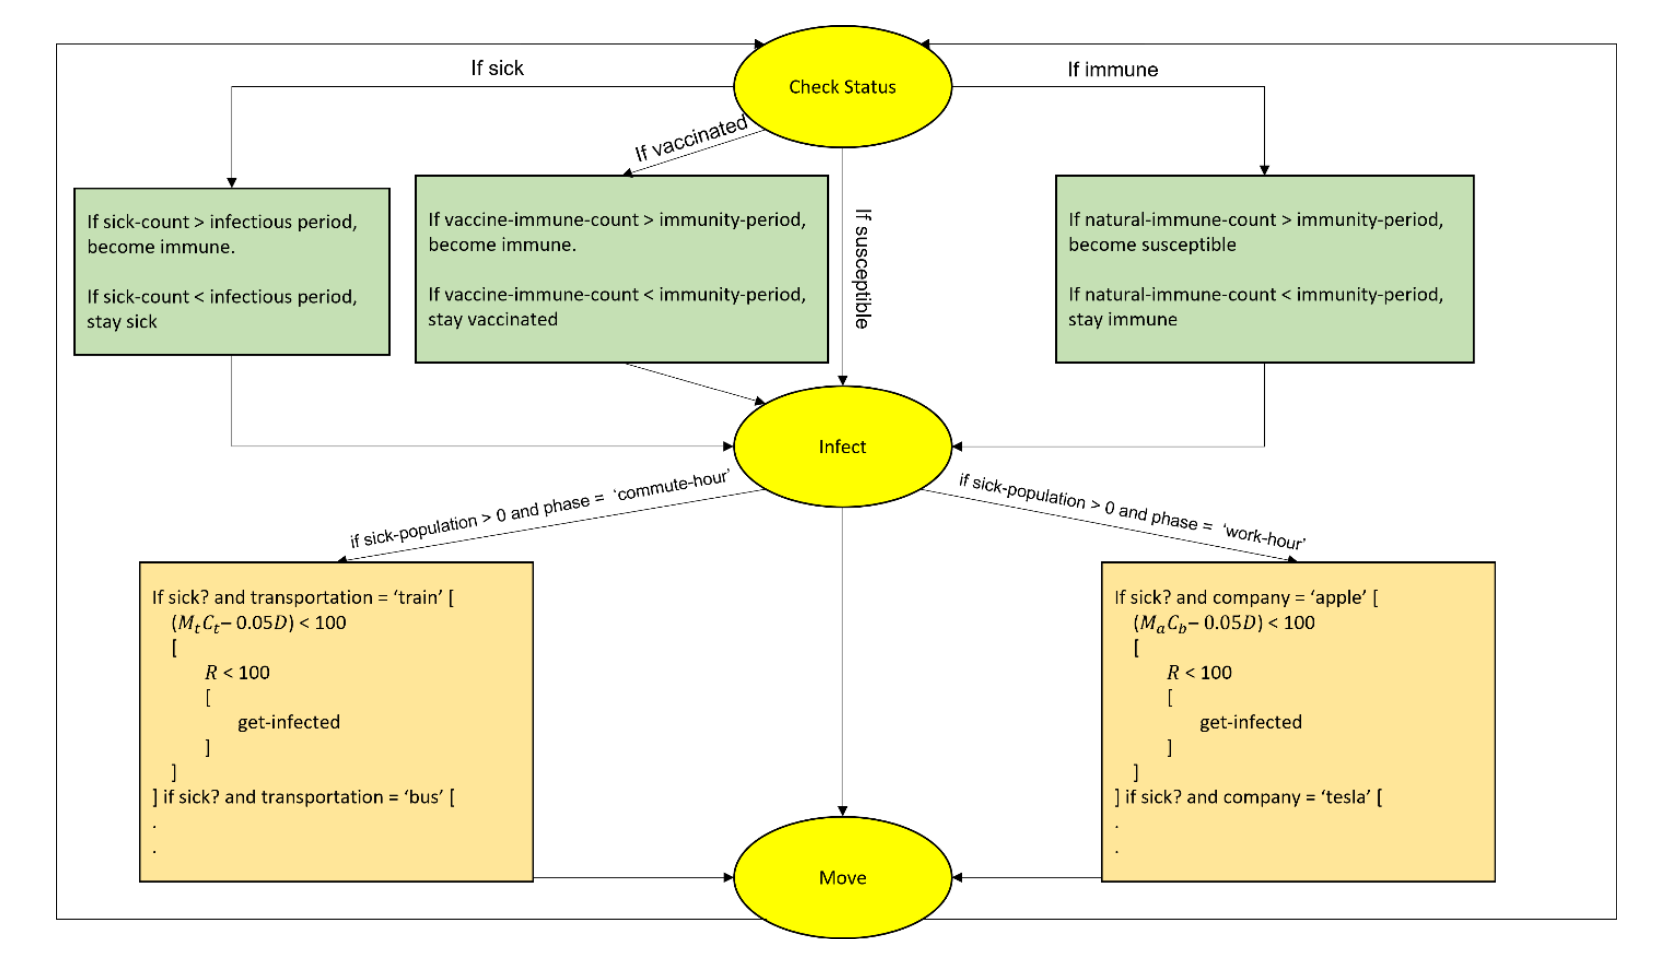
\includegraphics[width=\linewidth]{figures/modelDynamics.png}
	\caption{Description of model dynamics. Processes are described using the NetLogo syntax, as used in the model implementation.\label{fig:modeldyn}}% rq: should also redo fig for no netlogo? diffcult at this level of granularity
\end{figure}


\subsection{Model parametrisation}

We give in this section more details on the parametrisation of the stylised model.

%All variables are shown in Fig.~\ref{fig:modelvars} (see the open implementation and code linked below).
%\begin{figure}
%	\centering
%	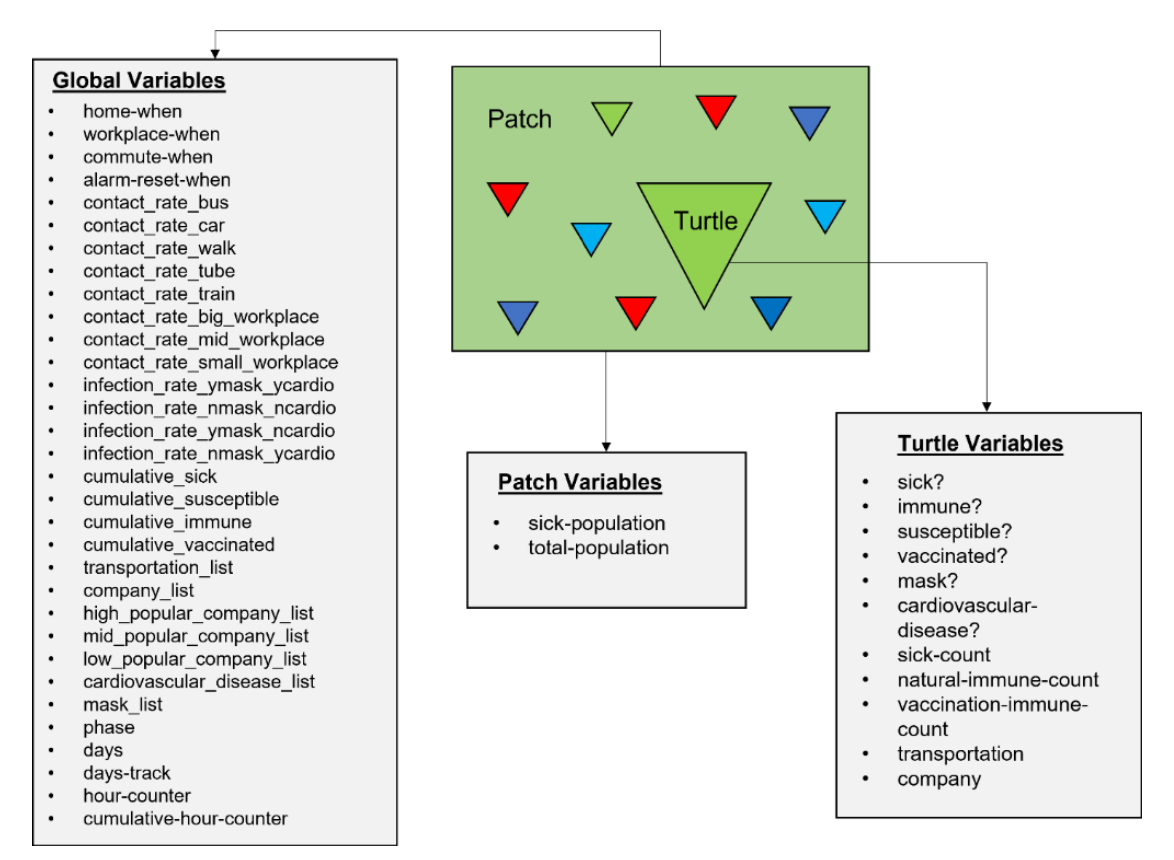
\includegraphics[width=\linewidth]{figures/ModelVariables.png}
%	\caption{Model variables \label{fig:modelvars}}	
%\end{figure}



\subsubsection{Global variables}

Infection rates are calculated based on global and local parameters. The variables that define contact rates for each mode of transportation and company are pre-defined with specific values.

For transportation contact rates, we take stylised values decreasing with the density one can expect in each transport mode: $c_{bus} = 40\%$, $c_{metro} = 35\%$, $c_{train} = 30\%$, $c_{walk} = 10\%$, $c_{car} = 0\%$.

No discrete values define the accurate contact rates for different modes of transportation, but the general assumption was made based on the understanding that the lower the capacity of transportation, the higher the density; hence, the higher contact rates between the passengers. The contact rate specifically for the car is set to zero because it is assumed that an agent who commutes by a car makes no contact with other agents during the 'Commute-hour' phase. The same logic was applied when defining the contact rates for different companies. The assumption was based on the understanding that the bigger the company size, the more the agents interact.

For contact rates on work site, we therefore take the following values: $c_{Big} = 40\%$, $c_{Medium} = 35\%$, $c_{Small} = 30\%$. These values do not have an empirical basis, and should be integrated in the sensitivity analysis, would the model be applied to a real-world decision making problem (in the following, we provide only a proof-of-concept with few other parameters).


\subsubsection{Agent variables}


The importance of wearing a mask while interacting with an infected agent can significantly reduce the chance of infection. Furthermore, patients with cardiovascular diseases are possibly with a higher risk of getting an infection \cite{ielapi2020cardiovascular} (this aspect could also capture individuals with a deficient immune system for example). Due to these reasons, we have pre-defined values for infection risk rates based on the combination of these two variables: No mask \& Cardio = 50\% risk rate; Mask \& Cardio = 45\%; No mask \& No cardio = 15\%; Mask \& No Cardio = 10\%. We do not consider the fatality of the disease, but these would follow similar patterns.


% not necessary
%\subsubsection{Patch variables}
% sick population
% total population
%For each patch, the values of the sick and the total population get updated constantly. If the value of the sick population gets bigger than zero, the infection process between the agents within that specific patch gets triggered.


\subsection{Model parameters}


We list below main model parameters which will vary during numerical experiments, corresponding to the processes on which the model focuses.

\begin{itemize}
	\item Infectious period, ranging from 2 to 4 weeks; the longevity of the infectious period of an agent is believed to play an essential role in the spread of diseases because the longer the infected agent stays contagious, the more the chance of infection during an extended amount of time \cite{wilkinson2018impact}.
	\item Immunity period, ranging from 9 to 11 months. This is selected as one of the model’s input parameters because it is believed to play a vital role in protecting the agents from infection \cite{reyes2016modeling}. Hence, we are interested to know to what extent the immunity period significantly affects the spread of diseases.
	\item Vaccination rate: as discussed in the literature review, vaccines are the most effective preventive measure which can trigger a biological immune response to fight disease-causing organisms: beside strongly reducing the fatal outcomes, they also induce a decrease in infection rates (variable depending on diseases and vaccines, for example some estimates of effectiveness against infection on particular Covid-19 variants and vaccines were mainly above 50\% 30 days after injection \cite{mohammed2022efficacy}). The value ranges from 0 to 0.5 \%, meaning from 0 to 0.5 \% of the susceptible population is set to be vaccinated daily. A high vaccination rate is strongly believed to be the key to a successful control of epidemics; hence, finding out the impacts of different vaccination rates on the overall infection process is meaningful.
	\item Social distancing level: a certain level of social distancing is being applied by governments worldwide, hoping to stop the spread of diseases like COVID-19. However, the effect of social distancing is not yet well known. Due to this, it would be an interesting experiment to find out the effectiveness of such measures on disease transmission dynamics. The level of social distancing ranges from 1 to 3. Each level refers to a percentage value that reduces the contact rate by 5. Hence, the actual percentage value of the social distancing ranges from 5 to 15 percent. The higher the intensity of social distancing, the lesser the chance people contact each other. In practice, quantifying social distancing is complicated \cite{caley2008quantifying}, thus this stylised mechanism which should be refined in case of a practical policy application of our model.
\end{itemize}



\subsection{Model indicators}


As mentioned previously, the ABM is constructed following a structure similar to the SIRV compartmental model. Therefore, the indicators consist of proportional numbers of agents in each compartment, including susceptible, infected, recovered, and vaccinated.

%For demonstration purposes, we also calculate the infection rate for agents who commute by train during the 'Commute-hour' phase and the infection rate for agents who work in the 'Apple' company during the 'Work-hour' phase.





\subsection{Model implementation and exploration}

The model is implemented in NetLogo, which is a reasonable choice for such hybrid models in which visualisation is important. It is integrated into the OpenMOLE platform for model exploration \cite{reuillon2013openmole} to carry out the numerical experiments described below. Source code of the model and exploration scripts are openly available on a git repository at \texttt{https://github.com/henry-kang-7/CASA0004}.


The pre-defined input parameter values of the model are the following: infectious-period $\in \{ 2, 3, 4 )\}$ (weeks); immunity-period $\in \{ 4, 5, 6  )\}$ (months); vaccination-rate $\in \{ 0, 0.25, 0.5 \}$ (\%); social-distancing-levels $\in \{1, 2, 3\}$ (levels).

This results in 81 different combinations of the input parameter values for a grid sampling. The model is set to run over 125 times for every combination of the input parameter values, and the output parameters' average values are obtained at the end. The size of the 95\% confidence interval around the estimated average of a normal distribution of standard deviation $\sigma$, with $n$ replications, is given by $2\cdot 1.96 \cdot \sigma / \sqrt{n}$, and therefore $n=125$ ensures that the error on indicators is more than ten times smaller than the standard deviation.



\section{Results}


We describe now numerical results obtained through the extensive exploration with the OpenMOLE platform.


\subsection{Statistical distribution of indicators}

The LHS (Latin hypercube Sampling) method was used to explore the input space of the model. A total of 10,000 samples were drawn during the process (corresponding to 4 days and 4h of CPU time for model execution), used to study statistical properties of model indicators.



\begin{figure}
	\centering
	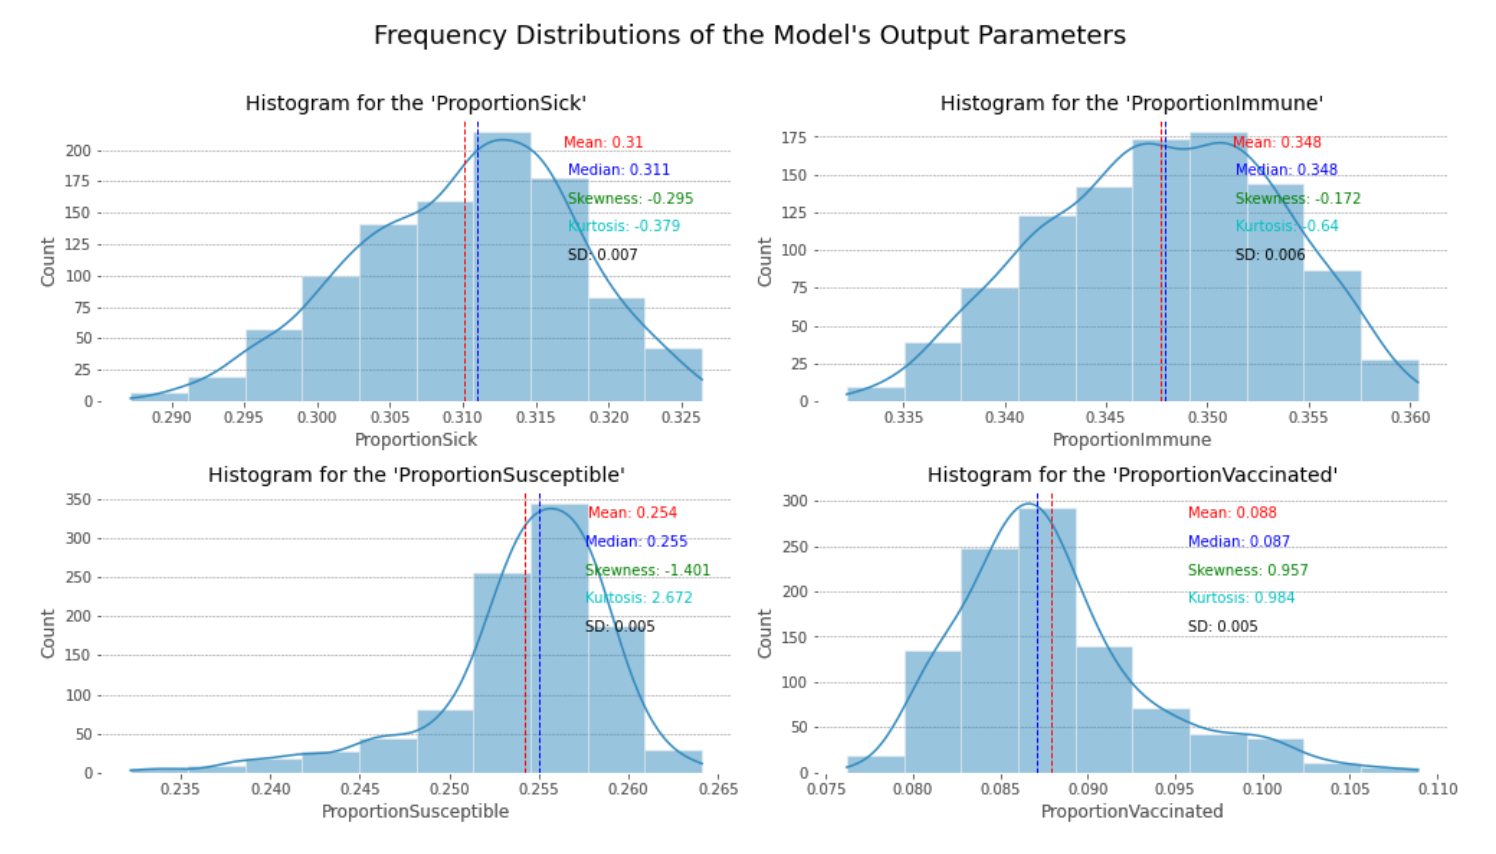
\includegraphics[width=\linewidth]{figures/histograms.png}
	\caption{Histograms of model outputs.\label{fig:histograms}}
\end{figure}

The histograms in Fig.~\ref{fig:histograms} illustrate the four different output indicators of the model. The histograms in the upper row comprise the 'ProportionSick' and the 'ProportionImmune' histograms, which appear symmetrical, but the skewness values indicate the traits of negative skewness on each histogram plot. Both kurtosis values are negative, suggesting that the distributions are thin-tailed. From this finding, we can assume that they generally follow characteristics of the platykurtic distribution. The 'ProportionSusceptible' and the 'ProportionVaccinated' histograms in the lower row appear negatively and positively skewed, respectively. The 'ProportionSusceptible' histogram is highly skewed to the left, which is indicated by the skewness value lesser than -1, while the 'ProportionVaccinated' histogram appears moderately skewed to the right as its skewness value is lower than 1. Furthermore, the kurtosis values of the two histograms are positive, which indicates that they both have heavier tails and are likely to follow the shape of the leptokurtic distribution.


% Figure 10 : qq plots
% The QQ plots shown in Figure 10 compare statistical distributions of the output parameters of the model relative to normal distribution. The shape of the ‘ProportionSick’ distribution closely follows the normal distribution but gets steeper towards the right. The ‘ProportionImmune’ distribution resembles the 'S-shaped trajectory of the data points. This implies that the distribution has thinner tails on both sides, shaping the distribution narrower compared to the normal distribution. The ‘ProportionSusceptible’ and ‘ProportionVaccianted’ data points resemble concave downward and upward shapes relative to the normal distribution line, respectively. This implies that the former distribution is negatively skewed, and the latter is positively skewed.


\begin{figure}
	\centering
	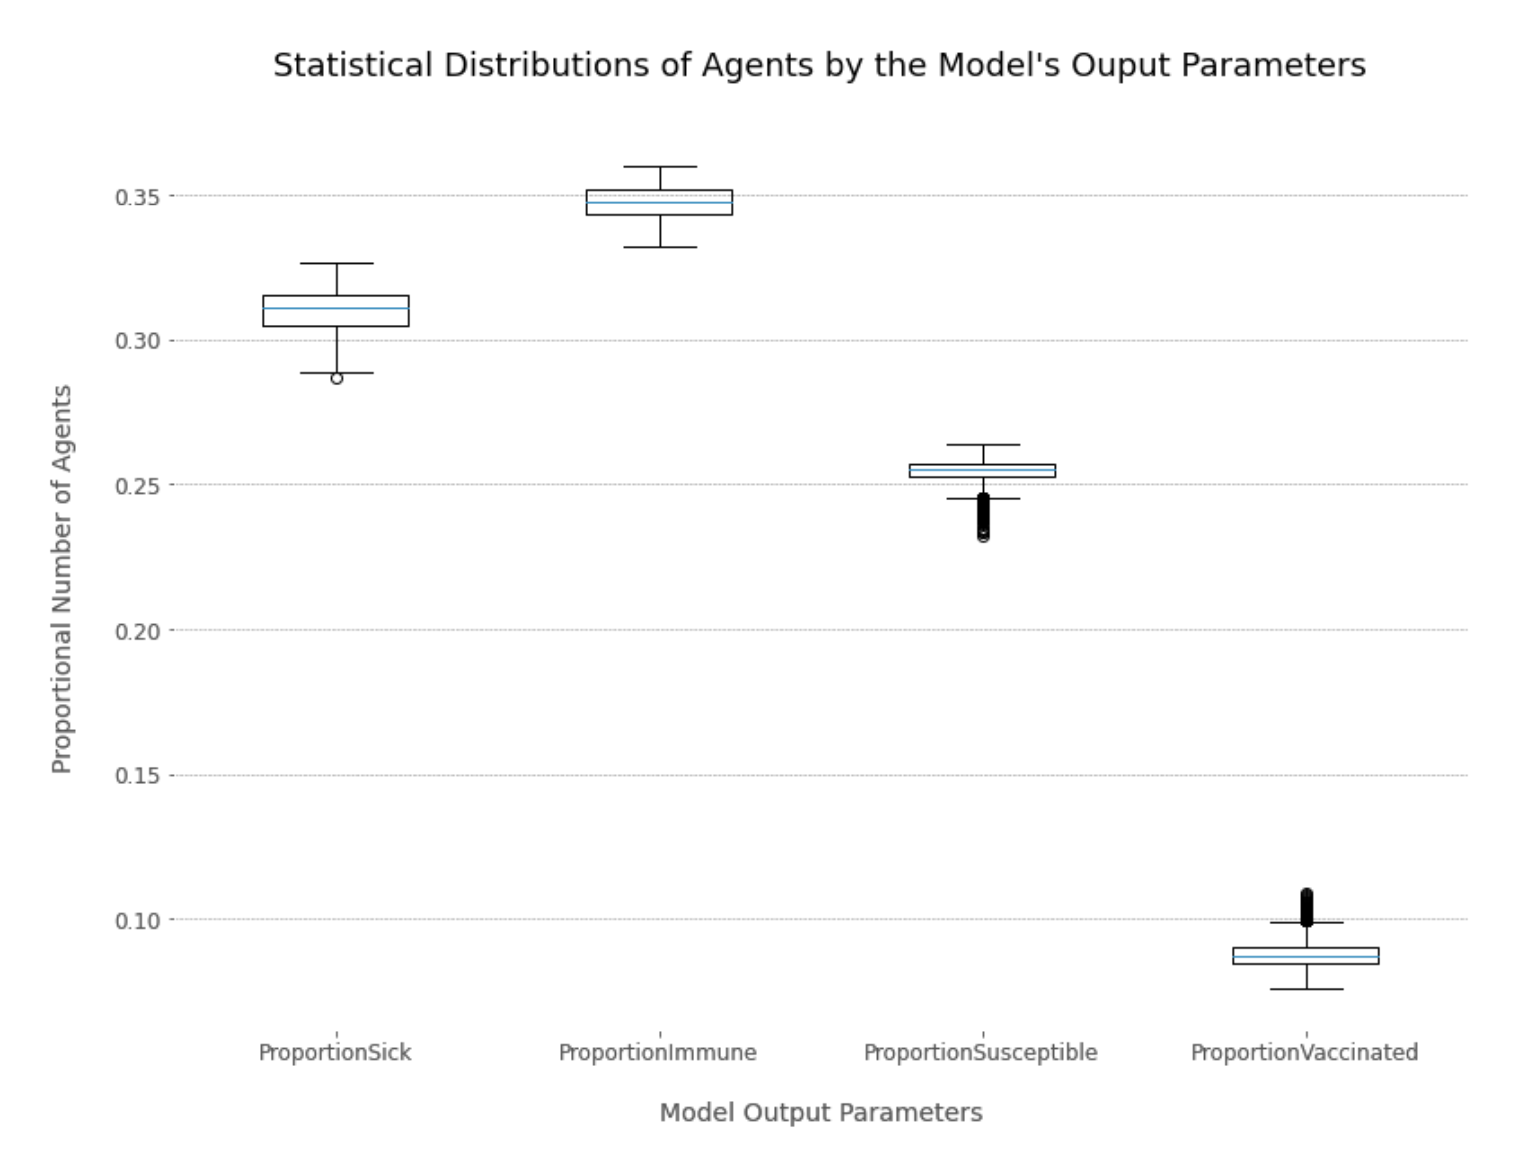
\includegraphics[width=\linewidth]{figures/agentTypeDistrib.png}
	\caption{Box plots of model outputs\label{fig:agenttypedistrib}}
\end{figure}


The boxplots presented in Fig.~\ref{fig:agenttypedistrib} show different data ranges and medians of the four different output parameters of the model. The boxplot representing the 'ProportionImmune' appears to have the highest median among the groups, followed by the 'ProportionSick', 'ProportionSusceptible' and 'ProportionVaccinated', respectively. Outliers in the boxplots are present regarding the 'ProportionSusceptible' and 'ProportionVaccinated'. Based on the histograms shown in Fig.~\ref{fig:histograms}, these distributions have positive kurtosis values and are disproportionally distributed, indicating low standard deviation; hence, high chance of producing outliers.


\subsection{Grid exploration}

The total combination of the model's input parameters with predefined values is 81. The model run for each combination of the inputs is set to 125 times as explained previously. This results in 10,125 model runs, for a total execution time of 4 days and 5 hours.

%Table 6 presents the combinations of the input parameter values relative to the five lowest values of the ‘ProportionSick’. The lowest value of the ‘ProportionSick’ among the 10,000 samples is 0.2779. The combination of the input parameter values that generated the lowest ‘ProportionSick’ is shown in the first row of the table. The ‘infectiousPeriod’ and the ‘vaccinationRate’ values remained constant at 2 (weeks) and 0.005 (0.5\%) respectively, while the ‘immunityPeriod’ and the ‘socialDistancingLevels’ varied throughout the table.
%Table 7 presents the combinations of the input parameter values relative to the five highest values of the ‘ProportionSick’. According to this table, the highest value of the ‘ProportionSick’ among the 10,000 samples is 0.3280. The ‘infectiousPeriod’ and the ‘vaccinationRate’ remained constant at 4 (weeks) and 0.0 (\%), respectively, while the rest of the input parameter values varied throughout the table.




\begin{figure}
	\centering
	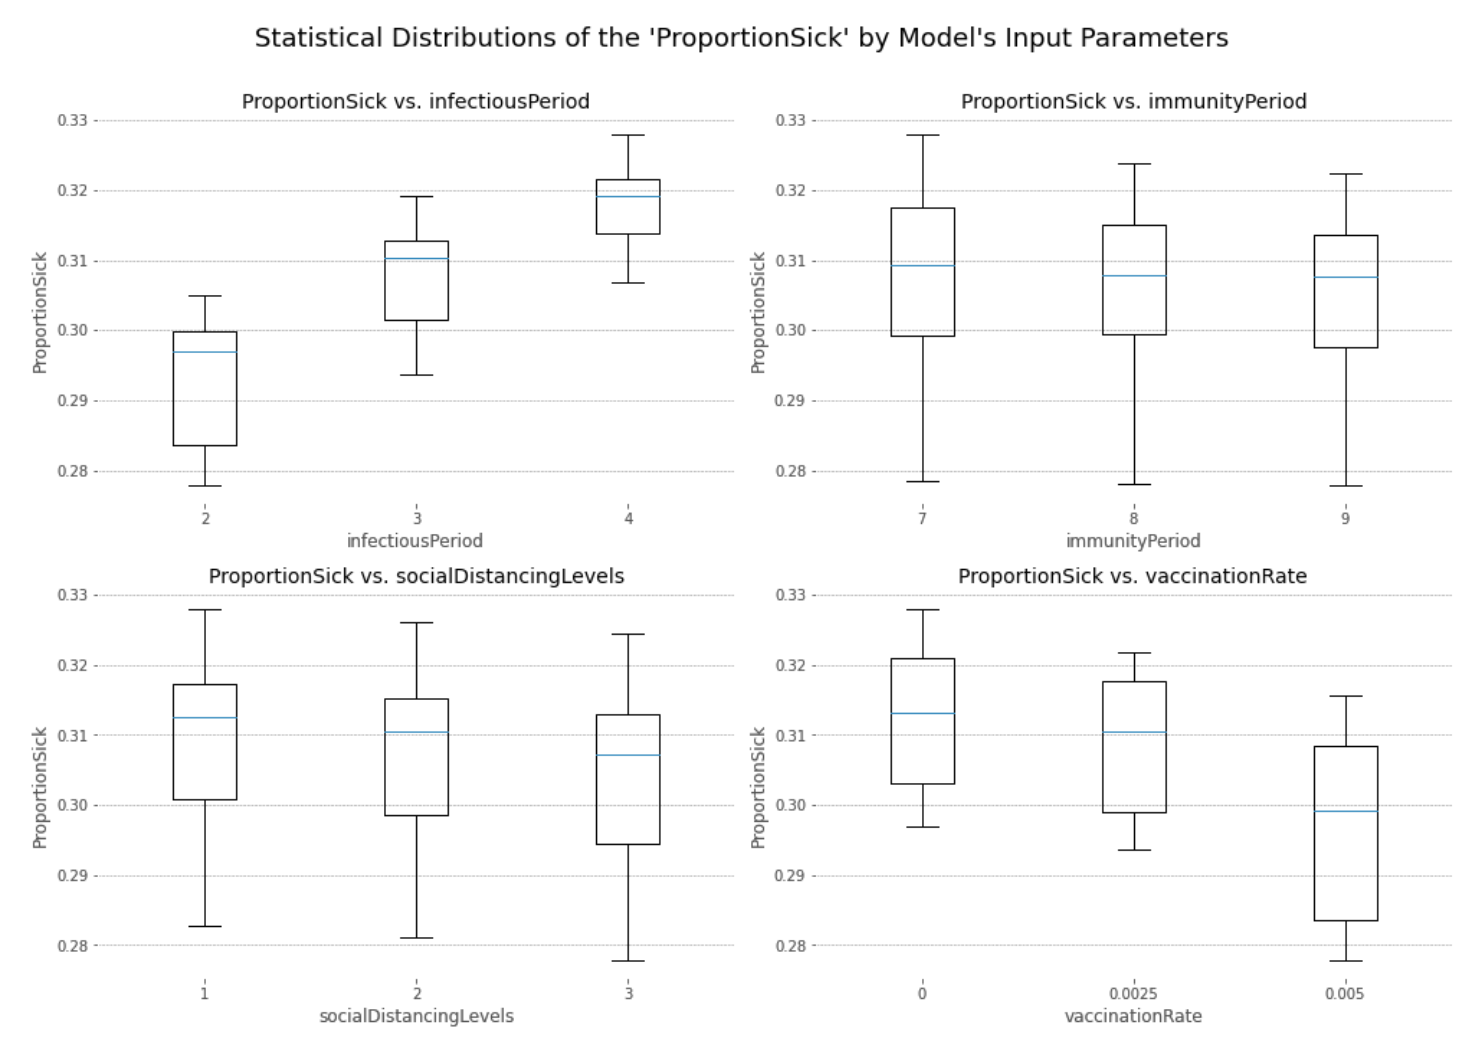
\includegraphics[width=\linewidth]{figures/boxplots.png}
	\caption{Box plots showing aggregate values of model outputs based on each value of inputs.\label{fig:boxplots}}
\end{figure}


The box plots in Fig.~\ref{fig:boxplots} show statistical distributions of the 'ProportionSick', which are grouped by each input parameter value of the model. The range of each input parameter is indicated on the horizontal axis of the graphs. The first graph represents the grouped values of the 'ProportionSick' by the values of the 'infectiousPeriod'. It indicates that a unit increase in the infectiousPeriod' value increases the boxplot's overall median and max values. The boxplots related to the 'immunityPeriod' and the 'socialDistancingLevels' show a marginal decrease in the median of the boxplots per unit increase. The last graph is related to the 'vaccinationRate', which indicates that a 0.0025 (0.25 \%) increase in the rate decreases the boxplot’s overall values. It indicates that vaccines have an apparent effect on successfully controlling the spread of diseases.


\begin{figure}
	\centering
	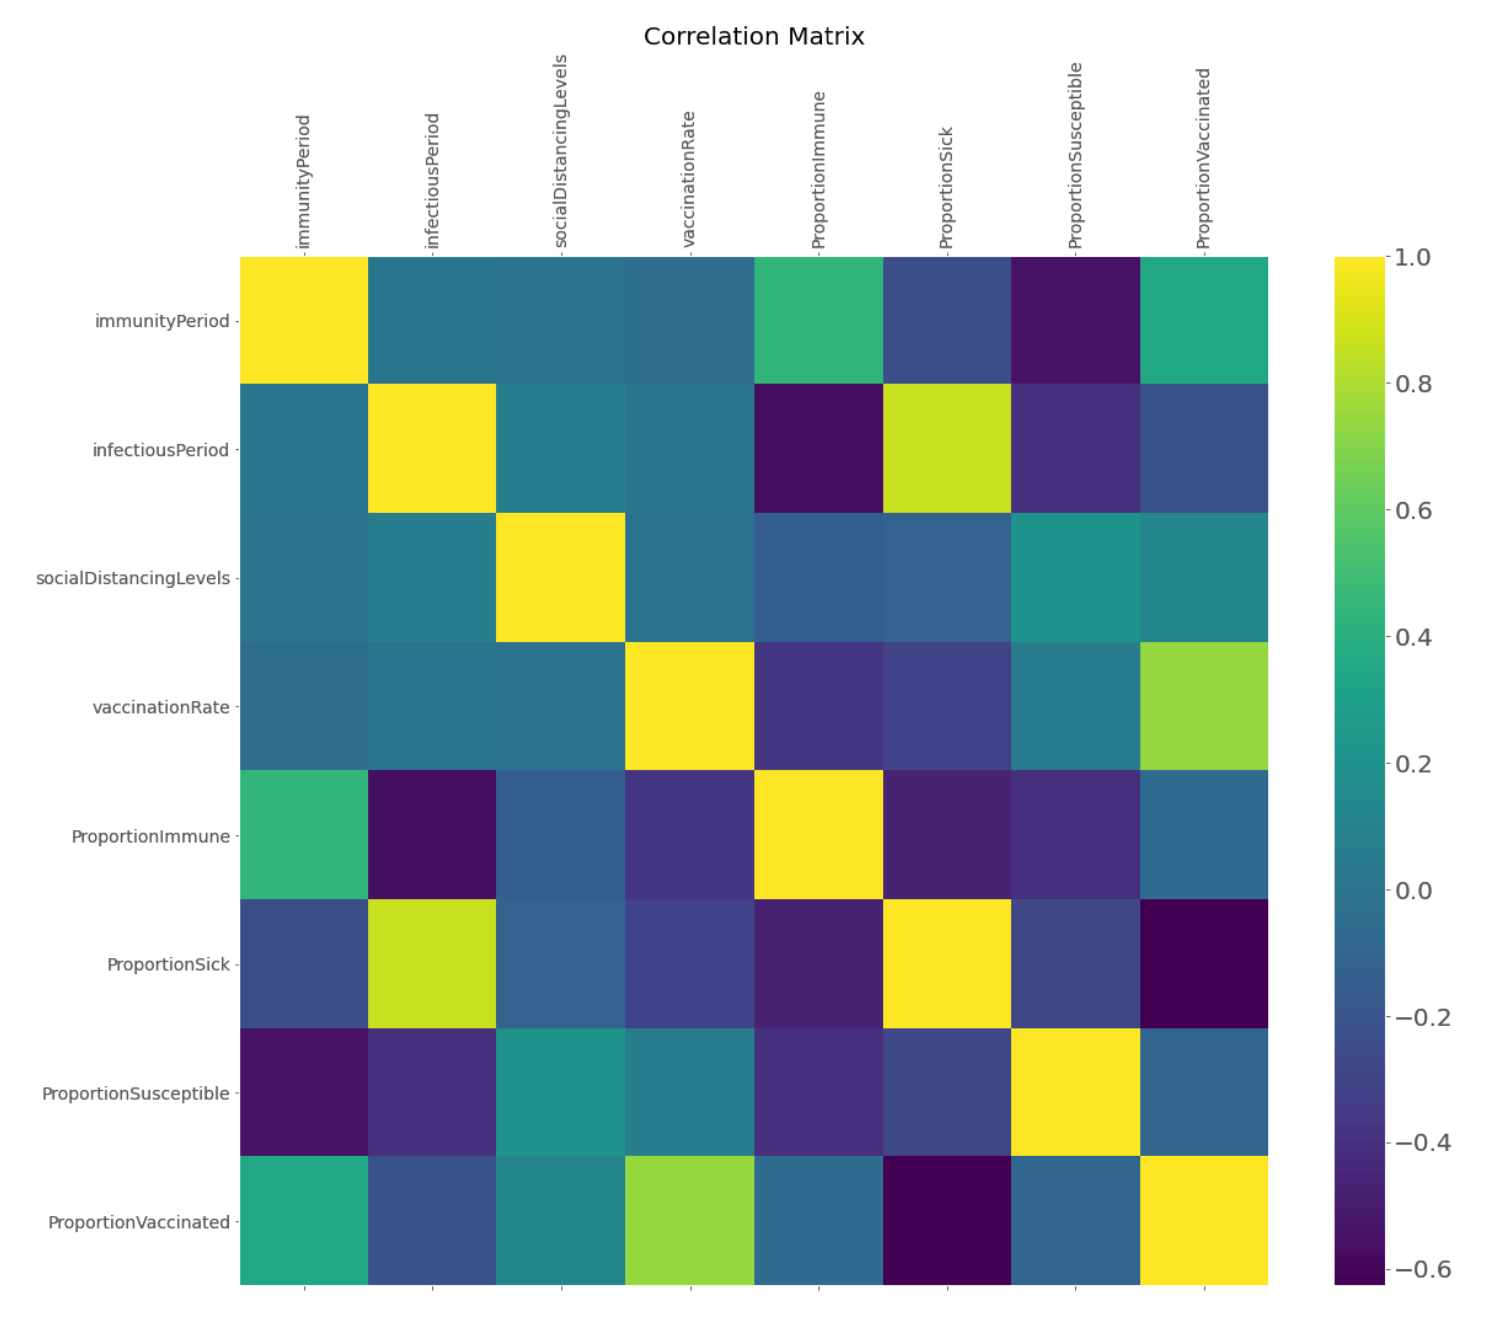
\includegraphics[width=\linewidth]{figures/correlations.png}
	\caption{Correlation matrix of model parameters and indicators.\label{fig:correlations}}
\end{figure}


The correlation matrix illustrated in Fig.~\ref{fig:correlations} displays the correlation between different model parameters. The 'ProportionSick' and the 'infectiousPeriod' appear to be highly correlated. According to the box plots shown in Fig.~\ref{fig:boxplots}, every unit increase in the 'infectiousPeriod' also increased the 'ProportionSick' values. The rest of the input parameters, including the 'immunityPeriod', 'socialDistancingLevels' and 'vaccinationRate' are negatively correlated with the 'ProportionSick' at different intensity levels.

%The dependent variable of the regression summary shown in Figure 16 is the ‘ProportionSick’. All four input parameters of the model indicate significant p-values of zero, and the R-squared value is 93.7\%. The highest and the only positive coefficient among the four input parameters is between the ‘ProportionSick’ and the ‘infectiousPeriod’ by 0.0115. It indicates an increase in ‘ProportionSick’ by 0.0115 for every unit increase in the value of the ‘infectiousPeriod’. On the other hand, the coefficient values of the ‘immunityPeriod’, ‘socialDistancingLevels’ and ‘vaccinationRate’ are all negative by -0.0033, -0.0023 and -0.0041, respectively.
%In this research, we used multiple linear regression to estimate the relationship between the model’s input parameters and the proportional number of sick agents. A supplementary correlation matrix is drawn to visualise how strong the model parameters are correlated with each other.

An OLS regression with the simulated data shows that the spread of infection mainly depends on the longevity of the infectious period. The longevity of the infectious period plays a vital role in disease transmission because a more extended infectious period allows an infected agent to interact with a more significant number of susceptible agents for an extended time. For example, an infected agent who is infectious for a single day is unlikely to infect a more significant number of susceptible agents than an infected agent who is infectious for a week. A more extended infectious period is, therefore, a dangerous factor that may rapidly increase the chances of infections, often creating a mass infection wave.

\subsection{Model surrogate}

Then, a random forest model is trained with the original data obtained by the LHS method during the first step of the analysis to forecast the proportional number of sick agents. This supervised machine learning method is versatile, easy to use and train, but also provides interpretable results on the relative importance of features, and we use it for these reasons.

In order to train the random forest model to predict the values of the 'ProportionSick', the original data is categorised into train, test, and validation data in the ratio of 7:1.5:1.5. Before fitting the model with the train data, various numbers of trees with their corresponding accuracy scores are calculated. Then, this hyper-parameter for the model was optimised using the grid search method for a given set of estimator values, including 800, 900, 950, 1000 and 1050. As a result, 900 is the best value for optimising the random forest model. The random forest with the 900 decision trees was developed by fitting the training data to predict the values of the 'ProportionSick' and including all four input parameters of the model.

%The predicted values of the 'ProportionSick' via the random forest are compared with the actual values in a table. The comparison between the statistical distributions of those two types of values is then visualised on a density plot.

We obtain a MAE (how big of an error we can expect from the forecast on average) of 0.001, which implies that the average errors between the predicted and actual values are marginal; hence, the predictions are considered highly accurate. Moving on to the MAPE, the value of 0.363 indicates that, on average, the forecast is off by 0.363\%. This means that the accuracy of the forecast is as high as 99.637\%. Lastly, the value of the RMSE is also 0.001, which indicates that the difference between the predicted and actual values is marginal.

\begin{figure}
	\centering
	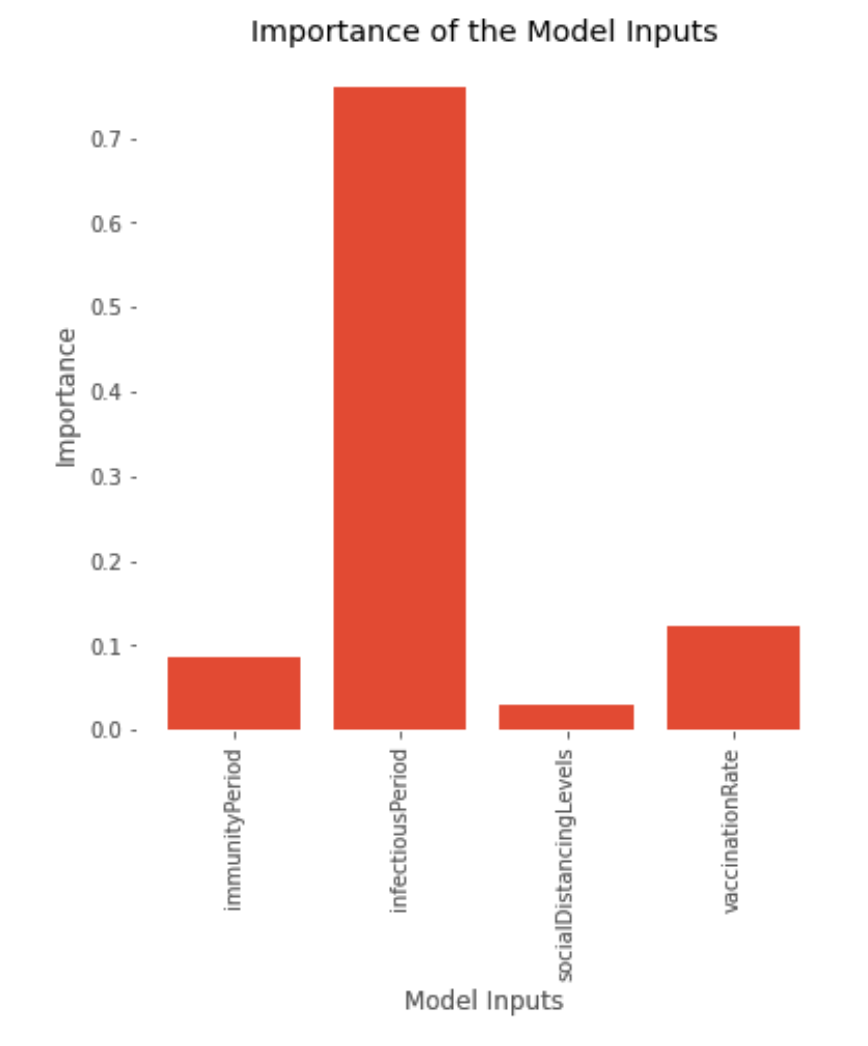
\includegraphics[width=0.7\linewidth]{figures/randomForest.png}
	\caption{Feature importance of input parameters obtained with the random forest surrogate.\label{fig:randomForest}}
\end{figure}


The random forest model is furthermore useful to quantify the importance of the model's input parameters, shown in Fig.~\ref{fig:randomForest}. The 'infectiousPeriod' is by far the most significant input parameter of the model, with a value of approximately 0.75, followed by the 'vaccinationRate' with a value of slightly over 0.1. The 'immunityPeriod' and the 'socialDistancingLevels' have an importance rate below 0.1, showing less importance than the previous two parameters.


\subsection{Global sensitivity analysis}

The previous results of parameter importance can be compared with an other method to quantify parameter's influence on indicators. The global sensitivity analysis method, introduced by \cite{saltelli2008global}, gives a broad summary of such an influence. In order to generate an accurate result for the sensitivity analysis, a total of 60,000 samples were run (25 days 7 hours of model runtime).

\begin{table}
\caption{Saltelli total order indices}
\begin{tabular}{|c|c|c|c|c|}
Outputs & infectiousPeriod & immunityPeriod & vaccinationRate & socialDistancingLevels\\
ProportionImmune & 0.72 & 0.333 & 0.665 & 0.7\\
ProportionSick & 0.692 & 0.09 & 0.365 & 0.143\\
ProportionVaccinated & 0.516 & 0.319 & 0.587 & 0.337\\
ProportionSusceptible & 0.341 & 0.066 & 0.92 & 0.277\\
\end{tabular}
\end{table}

The total-order indices shown above indicate that the 'infectiousPeriod' has the most significant impact on the values of the 'ProportionSick' followed by the 'vaccinationRate', 'socialDistancingLevels' and 'immunityPeriod' respectively. We find a very low effect of the immunity period on the proportion of sick and susceptible, meaning that uncertainties on this value will have a limited impact. The vaccination rate is also a critical input parameter of the model that plays a vital role in controlling the spread of diseases because the vaccine is a significant source of protective measures that can effectively stop viruses from transmitting one agent to another \cite{storlie2021quantifying}.



\subsection{Multi-objective model optimisation}

In attempting to control the spread of epidemics, many problems involve multiple objectives which cannot simply be described as the more, the better or the lesser, the better; instead, each objective has an ideal target value, and the main goal is to be as close as possible of the targeted value. To optimise the values of the input parameters, we define two objectives that are expected to be minimised. Firstly, we expect the proportional number of sick agents to be optimised, which is directly linked to the main interest of our research question. Secondly, we expect the proportional number of vaccinated agents to be optimised. Vaccination is a primary preventive measure that plays a vital role in successfully controlling the spread of diseases and even has the potential to achieve herd immunity, while other measures such as social distancing can only slow down the process of disease spreading instead of stopping them \cite{bicher2022model}. However, vaccines are not always available for multiple reasons, such as the high manufacturing and transportation costs \cite{plotkin2017complexity}. This is where decision-makers often face a dilemma because attempting to control epidemics will cost money and the best option which they might have at this point is to find a good balance between the use of vaccines and the proportional number of sick agents, respecting the economic budget.

The way to find the results that provide a good approximation of the Pareto frontier with acceptable trade-offs between the identified objectives is by using the NSGAII algorithm. The NSGAII is a commonly used type of multi-objective optimisation algorithm which includes a fast non-dominated sorting, crowding distance assignment and a sorting procedure \cite{deb2002fast}.

The Pareto Front consisting of non-dominated solutions relative to the 'ProportionSick' and 'ProportionVaccinated' is drawn after running a total of 10,000 generations of the OpenMOLE implementation of the algorithm.
%3 days 19 hours = 3.79 days


\begin{figure}
	\centering
	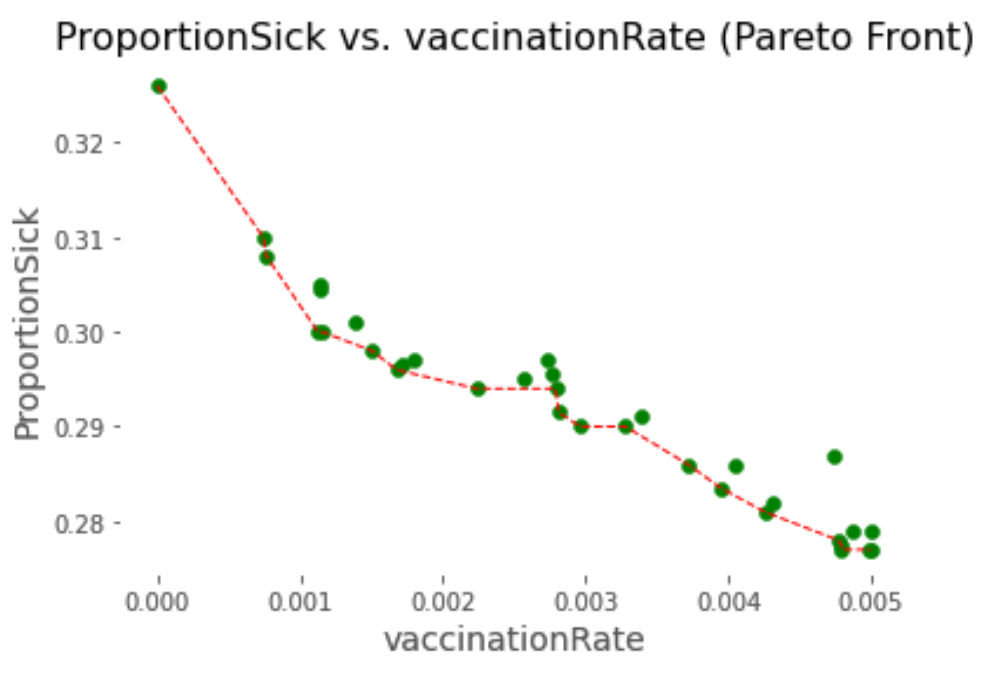
\includegraphics[width=\linewidth]{figures/pareto.png}
	\caption{Pareto front of proportion of sick vs. vaccination rate.\label{fig:pareto}}	
\end{figure}

The Pareto Front shown in Fig.~\ref{fig:pareto} illustrates the optimal solution set of the 'ProportionSick' and the 'vaccinationRate' as two objectives. The value of the 'ProportionSick' appears to decrease rapidly as the value of the 'vaccinationRate' increases. The slope of the line is generally steep throughout the graph. Plus, the difference between the values of the 'ProportionSick' with and without the vaccination is clear. The non-linearity of the front is an interesting feature, witnessing the underlying complexity when exploring policy trade-offs.


\begin{figure}
	\centering
	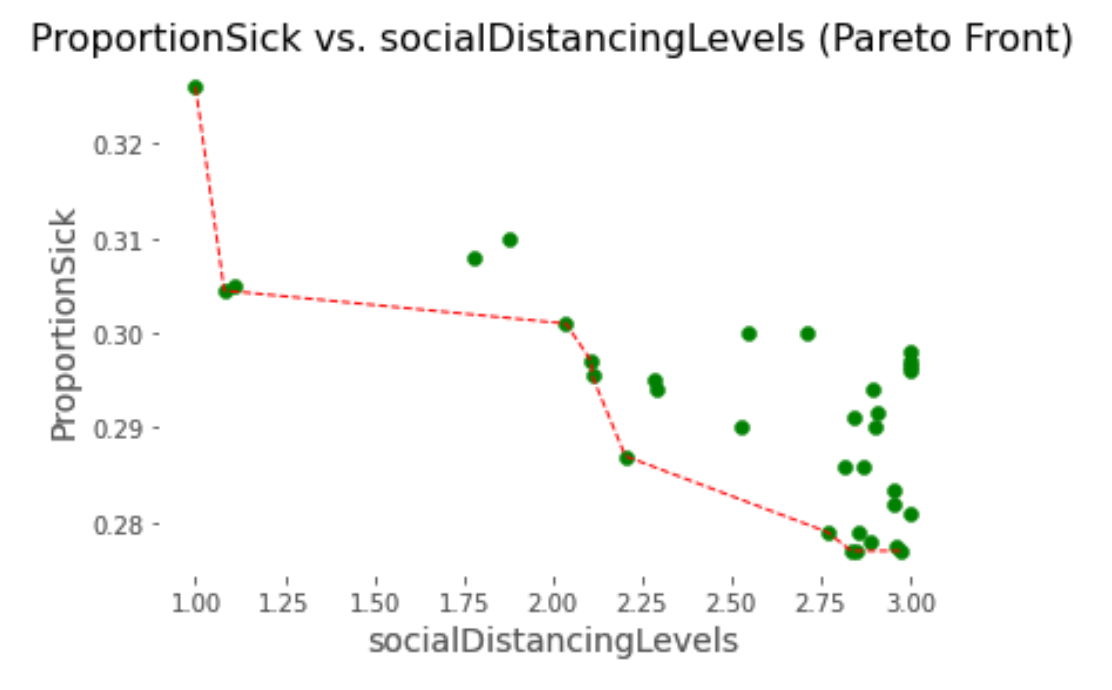
\includegraphics[width=\linewidth]{figures/pareto2.png}
	\caption{Pareto front of proportion of sick vs. social distancing levels.\label{fig:pareto2}}	
\end{figure}



The Pareto Front, visualised in Fig.~\ref{fig:pareto2}, is formed with the optimal values of the 'ProportionSick' and the 'socialDistancingLevels' as two objectives. It indicates a clear sign of a decrease in the value of the 'ProportionSick' as the value of the 'socialDistancingLevels' increases. In some regions of the front, a quasi-vertical increase means that much control may be gained at a very low social cost, what has implications when finding the compromise between the epidemic impact and the social impact of lockdowns. The social distancing level is indeed an essential input parameter that acts as a preventive measure against infectious diseases in our model. Social distancing must be implemented with care because if the intensity is too high, it prohibits necessary human interactions, which reduces the productivity rate, negatively impacting the economy in general \cite{deluca2020unequal}. Due to this, finding a good balance between the social distancing level and the proportional number of sick agents would be essential in ensuring a healthy economy while keeping the number of infected cases low.


\section{Discussion}

The diverse numerical experiments, applying various model exploration and validation methods, can be used to provide useful policy insights in this stylised case. They are not directly applicable to real world situations, as a slightly more data-driven approach would be needed, but this already suggests how such methods can compensate for model simplifications. Thus, we suggest that our work is a proof-of-concept of how such systematic model exploration may hinder issues due to parameter uncertainty, or the lack of data, for similar epidemiological models.

Some limitations of this work can be given. First, the population size of the simulation had to be limited to a small number, mainly due to the expensive computational cost and time. In order to fasten the process, these executions have been distributed using OpenMOLE, but the limitation in the level of detail and granularity is a recurring issue with ABMs. We still need to investigate if the trade-off chosen here is reasonable.

The current number of input parameters is limited to only four parameters. However, there can be more numbers of input parameters introduced in our model to generate more dynamic results which can better reflect real-life situations. Furthermore, the current model can be extended with more compartments that can describe various states of an agent in the infection process, such as death or exposure \cite{reyne2022principles}. The model is also flexible in that it can add many more characteristics of agents, such as age, occupation, vaccination record and gender, which can be considered in the process of interaction and infection.

As a future work, regarding the stylised parametrisation taken here for several aspects of model setup, a more advanced sensitivity analysis relaxing these parameters could be done. More particularly, quantifying the role of geography (transport geography, but also company size distribution and locations), is an interesting prospect, as new methods to achieve this have recently been developed \cite{raimbault2019space}.


\section{Conclusion}

This study proposed various model assessment methods to explore results obtained with a stylised ABM we introduced, based on the SIRV compartmental model to study the spread of diseases. Through the model exploration, this study analysed the impacts of the pre-defined input parameters, which included the infectious period, immunity period, daily vaccination rate and social distancing level, on the spread of infectious diseases. We provide thus a proof-of-concept of how model exploration and validation methods can be a powerful tool to design and optimise health policies.



\bibliographystyle{spphys}
\bibliography{biblio}

\end{document}
